\hypertarget{h.ehus4lru41jz}{%
\section{\texorpdfstring{{DeVault - The Decentralized Social
Economy}}{DeVault - The Decentralized Social Economy}}\label{h.ehus4lru41jz}}

{Whitepaper Version 1.0 - October 2019}

{DeVault is a decentralized community and economy project. }

{Enriching the world 1 peer-to-peer transaction at a time.}

{\href{https://www.google.com/url?q=https://github.com/devaultcrypto\&sa=D\&ust=1574537005289000}{https://github.com/devaultcrypto/devault}}

{}

\hypertarget{h.ijvkyqh5t7oc}{%
\subsection{\texorpdfstring{{Introduction to The DeVault
Ethos}}{Introduction to The DeVault Ethos}}\label{h.ijvkyqh5t7oc}}

{The overarching goal of DeVault is to be}{~a '}{social digital
economy}{' for everyone, with the spirit of decentralization at the very
core. It will achieve this with a community governance system that
everyone has a voice in. To accomplish these goals we will be leveraging
a `}{D}{ecentralized }{A}{utonomous }{O}{rganization' }{(DAO)}{~schema
to scale up to 1+ million users for an online b2b and p2p focused,
crypto-oriented, social network. The social network Devault.online is
focused on user acquisition, personal growth and privacy.}

{}

{Devault.Online }{(and others)}{~will act as a portal into the digital
economy of DeVault.cc (the }{payment protocol}{~residing on a
blockchain}{). This will allow users to not only build out comprehensive
resume style profiles, but also provide many tools such as user driven
governance, the ability to friend and chat with users on the site and
will include business and community profile options. ~In the future
we'll have an achievement system to help further add to the value via
methods of gamification and community building.}

{}

{Some of the main goals of the project relate to creating a
fairly-distributed worldwide social network where users and power users
alike, can have the ability to earn and get deeply involved in the
crypto space without having prior knowledge of crypto. We plan to
leverage education to create and onboard for the entire space as well as
Devault.online itself.}

\hypertarget{h.844cfd63jvaa}{%
\subsection{\texorpdfstring{{Noteworthy Features of
DeVault}}{Noteworthy Features of DeVault}}\label{h.844cfd63jvaa}}

{These are the pertinent features of DeVault for those short on time to
read this document in full, they can click on the appropriate section}

{}

\begin{enumerate}
\tightlist
\item
  {\protect\hyperlink{h.c0d8fzly70q7}{Community Governance - 1 Coin = 1
  Vote with On-chain funding}}
\item
  {\protect\hyperlink{h.7imft9llrxlk}{Sharkflation for a fairer
  distribution}}
\item
  {\protect\hyperlink{h.xc6vji4r4g6e}{Cold Reward System}}
\item
  {\protect\hyperlink{h.h4zmjemhgqxi}{Bitcoin Cash 0.19 Clone}}
\item
  {\protect\hyperlink{h.93av7wuny8ba}{Information on funded DAOs}}
\end{enumerate}

{}

\begin{center}\rule{0.5\linewidth}{\linethickness}\end{center}

{}

\hypertarget{h.c0d8fzly70q7}{%
\subsection{\texorpdfstring{{Community Governance / 1 Coin = 1
Vote*}}{Community Governance / 1 Coin = 1 Vote*}}\label{h.c0d8fzly70q7}}

{*There shall always be a system in place that is both open source and
utilizes the majority approved voting mechanism which will start out as
1 coin = 1 vote, as always the community is free to adjust this later.}

\hypertarget{h.parxytnbp8ej}{%
\subsubsection{\texorpdfstring{{Community
Rights}}{Community Rights}}\label{h.parxytnbp8ej}}

{A document titled `Community Rights of the DeVault Blockchain' will be
initial groundwork for a community approved form of a standardized
ethos. }

\hypertarget{h.lbkc9p2n9j2l}{%
\subsubsection{\texorpdfstring{{REAL Community
Governance}}{REAL Community Governance}}\label{h.lbkc9p2n9j2l}}

{In DeVault we aim to create a system in which as many people as
possible have a voice, and equal footing in the community. By leveraging
a 1 coin = 1 vote concept and a fair distribution, we will create a much
more effective form of decentralized community governance. Miners will
still secure the networt., but we believe there are many players in the
ecosystem and we intend to get them involved as well. }

{}

{All important decisions pertaining to the DeVault Blockchain can and
will ~be openly discussed in the community. ~Proposals can be submitted
to get involved and help grow the future of the DeVault Economy! }

\hypertarget{h.6d4jukb50wg9}{%
\subsubsection{\texorpdfstring{{Treasury
Voting}}{Treasury Voting}}\label{h.6d4jukb50wg9}}

{(Community) }{Treasury Proposals are things that either individuals
would like funding for and/or concepts the community thinks funding
would be spent on outside of the general day to day work of the
sponsored DAOs. After a treasury vote is passed it will require ⅘ of
multi sig holders to get paid out to a users balance (as anti scam and
hack feature, but the multi sig votes should ultimately comply with
community votes). If a coordinator would like to submit a `de-funding'
proposal for a project they believe is a problem or a scam they are free
to do so.}

\hypertarget{h.nredut5j8boy}{%
\subsubsection{\texorpdfstring{{Community
Voting}}{Community Voting}}\label{h.nredut5j8boy}}

{Community (Core) Voting is to say the community would like to discuss
any specific subject and garner a better understanding of the consensus
within the network by asking the network of voters.}

\hypertarget{h.rkwe9l9v54p2}{%
\subsubsection{\texorpdfstring{{Signing
Messages}}{Signing Messages}}\label{h.rkwe9l9v54p2}}

{The method of which votes will be tallied is based upon the concept of
`signing a message' to the DeVault blockchain with an address that
contains coins. The amount of coins in the address for the entirety of
the voting period, that do not leave the address will be counted as
valid towards either a `Yes' or `No' Vote on any and all community
budget decisions in DeVault as well as Community Core Voting. Any user
can currently do this by simply using a desktop wallet such as the
}{DeVault Qt}{~once they have loaded the HD Seed into the wallet. }

{*Please note there are certain rules that may invalidate your vote such
as moving funds after a vote has been cast, until the proposal has
finalized. }

\hypertarget{h.vh4w65alghcu}{%
\subsubsection{\texorpdfstring{{Maintaining
Transparency}}{Maintaining Transparency}}\label{h.vh4w65alghcu}}

{We intend to be a front runner in transparency \& accountability. }

{}

{One way we will create transparency is to have all budget transactions
logged on a single webpage (e.g. accountant.devault.cc) for all team and
community budget payouts with signed messages pertaining to the purpose
of the payment.}

{}

{To ensure a smooth road early on these payments will always require ⅘
(this will scale up as we grow \# of DAOs) ~multi-signature operators to
approve regardless of community voting as an anti scam measure, but must
overwrite the community vote with a new proposal asking the community to
reconsider the proposal. }

\begin{center}\rule{0.5\linewidth}{\linethickness}\end{center}

\hypertarget{h.7imft9llrxlk}{%
\subsection{\texorpdfstring{{}}{}}\label{h.7imft9llrxlk}}

\hypertarget{h.ey1iifm4kamk}{%
\subsection{\texorpdfstring{{`Sharkflation' for a fairer
distribution}}{`Sharkflation' for a fairer distribution}}\label{h.ey1iifm4kamk}}

{Reference Material:
}{\href{https://www.google.com/url?q=https://github.com/devaultcrypto/devault/blob/develop/ColdRewards.md\&sa=D\&ust=1574537005295000}{https://github.com/devaultcrypto/devault/blob/develop/Inflation.md}}

{}

{The block reward will increase gradually from 500 DVT to approximately
750 DVT (\textasciitilde1400 including budgets) for the first 6 months
(131,490 blocks), peak and reverse downward until eventually stopping at
1 DVT per block after 750 years. Originally the peak would have occured
at 1 ½ years out but the community decided to shorten the ramp up period
via a vote.}

{}

{First 10 years of Mining, Budgets \& Cold Staking* Rewards:}

{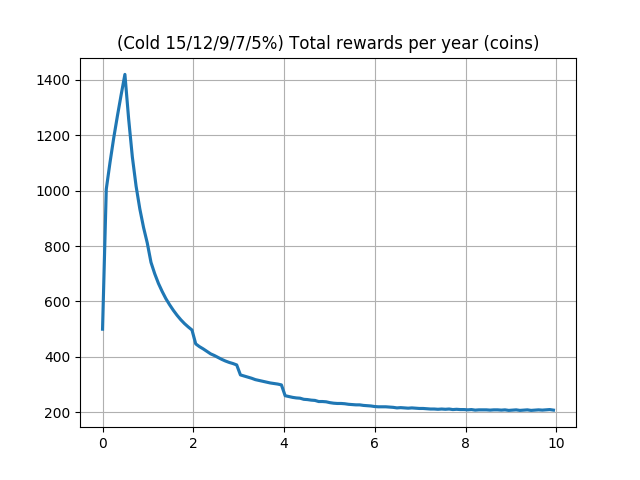
\includegraphics{images/image3.png}}

{*Assumed cold staking participation rate of 75\%.}

{}

{Total Supply after 10 years of Mining Rewards, Budgets \& Cold
Staking*:}

{}

{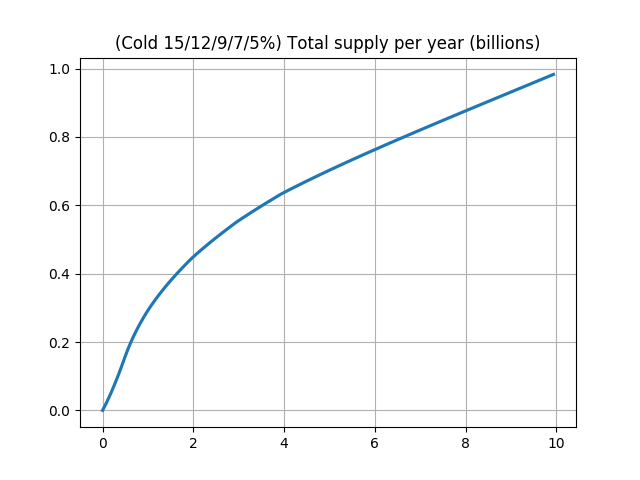
\includegraphics{images/image1.png}}

{*Assumed cold staking participation rate of 75\%.}

\hypertarget{h.xc6vji4r4g6e}{%
\subsection{\texorpdfstring{{Cold Rewards System
}}{Cold Rewards System }}\label{h.xc6vji4r4g6e}}

{Reference Material:
}{\href{https://www.google.com/url?q=https://github.com/devaultcrypto/devault/blob/develop/ColdRewards.md\&sa=D\&ust=1574537005297000}{https://github.com/devaultcrypto/devault/blob/develop/ColdRewards.md}}

\hypertarget{h.57rdcm3qxbam}{%
\subsubsection{\texorpdfstring{{Summary}}{Summary}}\label{h.57rdcm3qxbam}}

{Cold Rewards is a system to incentivize coin holders to hold coins for
at least a month in the same address. This helps to contribute to lower
sell pressure. How many coins can one receive by merely holding? This
changes yearly and starts at 15\% annualized. In the first year the
monthly rate is 1.25\% . So let's say Pete holds 100k DVT in his address
and doesn't spend any, the following month (21,915 blocks) he receives
1.25\% in Cold Rewards leading to a total balance of 101,250 coins, or
1250 coins in Cold Rewards.}

\hypertarget{h.s2r93qanslz8}{%
\subsubsection{\texorpdfstring{{Constraints}}{Constraints}}\label{h.s2r93qanslz8}}

{Cold Rewards pays out coins only to unspent transactions (UTXOs). What
are UTXOs? }{The analogy to~}{UTXO transaction model}{~would be paper
bills which you have in your wallet. In order to make a transaction of
\$1,000 (for example), your wallet should have at least \$1,000 in total
(after summing up all the bills). You can imagine each of these bills as
a UTXO. If you have a 10, and you get change for two 5s, you still have
10, but it's no longer in one UTXO. A}{t each new block, all of the
valid UTXOs will be evaluated for possible ColdReward payout. The
unspent transactions ~eligible for Cold Rewards must come from
``regular'' transactions. Mining rewards or previous Cold Rewards are
not be eligible. To calculate Cold Rewards, two things are taken into
consideration: (1) the difference between current BlockHeight (the block
number) and the BlockHeignt when the UTXO was created (let's call this
coin age) and (2) the BlockHeight when the UTXO got a reward last. The
coin address (UTXO) that is going to be rewarded (first) will be the one
with the highest `coin age'. If it so happens that multiple addresses
have the same coin age the largest one will get paid out. }

\hypertarget{h.4k4endzybkr}{%
\subsubsection{\texorpdfstring{{Minimum
Requirements}}{Minimum Requirements}}\label{h.4k4endzybkr}}

{25}{,000 DVT (rewards once a quarter), 21,915 blocks of holding
(starting after the 5th superblock, previously was 1000 DVT)}

\hypertarget{h.1igpojymhxgj}{%
\subsubsection{\texorpdfstring{{How to consolidate DVT into one
UTXO}}{How to consolidate DVT into one UTXO}}\label{h.1igpojymhxgj}}

{Now you know that your DVT must be stored in one UTXO of 25,000 DVT or
greater to accumulate Cold Rewards. And you know that if you mined DVT,
the payout you got from your mining pool is not eligible. So how do you
make it eligible? Easy.}

{In your DVT wallet, open the Settings menu, and click on Options, and
then the Wallet tab. Check the box to Enable coin control features and
then click okay. Click on the Receive button. Enter ``Cold Rewards'' or
whatever you want as the Label. Then click the New Address / Request
Payment button. A pop-up window shows up with a QR code. Click the Copy
Address button. Now click Send. Paste your new address into the Pay To
field. Click on the Inputs button on the top and click on Tree mode. The
address that your mining pool is sending your payouts to should be
visible there. Check the box next to it. Enter the amount (greater than
or equal to 25,000) that you want to set aside for Cold Rewards, and
click Send. You're done! You've consolidated your coins into one UTXO,
and as long as you don't spend coins from that UTXO, you will receive
Cold Rewards in about one month (after 21,915 new blocks have been
created). Using the Inputs button and selecting List mode, you can see
how many blocks have passed since you consolidated your coins. It's
listed in the Confirmations column.}

\hypertarget{h.1x0k649ygx22}{%
\subsubsection{\texorpdfstring{{Consolidating
Rewards}}{Consolidating Rewards}}\label{h.1x0k649ygx22}}

{In version 1.1 of the QT wallet, there is a Cold Rewards tab that gives
more information on the current state of UTXOs and rewards. Since Cold
Rewards that are paid out are not automatically eligible for Rewards
themselves (since they are coinbase transactions), they must be
consolidated into a new UTXO that is above the minimum of 25000 DVT. The
GUI page allows this to be done in an easy fashion. They can be combined
with previous UTXOs that have a low maturity percentage (i.e recently
paid out), so that the combined UTXO will yield a higher reward than
would happen without combining.}

{}

\begin{center}\rule{0.5\linewidth}{\linethickness}\end{center}

{}

\hypertarget{h.h4zmjemhgqxi}{%
\subsection{\texorpdfstring{{Bitcoin Cash 0.19
Clone}}{Bitcoin Cash 0.19 Clone}}\label{h.h4zmjemhgqxi}}

{Devault was started as a clone of Bitcoin Cash 0.19.0 which was
originally cloned from bitcoin around Bitcoin version 0.15. ~Our first
code commits were in Feb 2019 and there have been close to 700 commits
to date including various upstream updates to both Bitcoin and Bitcoin
Cash. }

{}

{As a clone of Bitcoin Cash, we have inherited some advantageous and
forward looking features}

{}

\begin{enumerate}
\tightlist
\item
  {Large Blocks - 32 Mbytes}
\item
  {Updated Schnorr signature support - not yet enabled}
\item
  {Avalanche consensus - not yet enabled}
\item
  {Re-org protection}
\item
  {Simple Ledge Protocol support - not used yet}
\item
  {Bech32 style addresses}
\end{enumerate}

{}

{Changes that improves the user experience}

{}

\begin{enumerate}
\tightlist
\item
  {Wallets are always encrypted with a password - for security benefit}
\item
  {HD enabled with Bip 29/39/44 supported mnemonic phrases that allow
  easy recovery and backup of private keys}
\item
  {Changes to Desktop wallets that allow for lightning fast setup and
  startup each time.}
\item
  {Reduction of decimal precision from 8 places to 3 places - also helps
  prevent spam transactions}
\item
  {Redesigned QT Wallet}
\item
  {Log files separated by date instead of everything in one file}
\end{enumerate}

{}

{Changes for an improved network}

{}

\begin{enumerate}
\setcounter{enumi}{6}
\tightlist
\item
  {Block times shortened from 10 minutes to 2 minutes for higher
  throughput}
\item
  {Use of LWMA difficulty algorithm for faster response to hash rate
  changes}
\end{enumerate}

{}

{}

{}

{}

{}

\begin{center}\rule{0.5\linewidth}{\linethickness}\end{center}

{}

\hypertarget{h.93av7wuny8ba}{%
\subsection{\texorpdfstring{{I}{nformation on funded
DAOs}}{Information on funded DAOs}}\label{h.93av7wuny8ba}}

\hypertarget{h.2ihr2nor4ixs}{%
\subsubsection{\texorpdfstring{{Funding
Split}}{Funding Split}}\label{h.2ihr2nor4ixs}}

{15\% - Community Treasury}

\hypertarget{h.6557snl66u3e}{%
\subsubsection{\texorpdfstring{{Team DAO Split
**}}{Team DAO Split **}}\label{h.6557snl66u3e}}

{Focus: core deliverables }

{10\% - Developer DAO }

{10\% - Web Developer/Support DAO }

{10\% - Business Development/Marketing DAO (}

{}

{**These splits can and should be adjusted from time to time by the
community consensus. Originally we had 5 team DAOs but after some team
members were no longer willing to help out, we consolidated down to 3.
For historical information on DAOs, please see github page}

{\href{https://www.google.com/url?q=https://github.com/devaultcrypto/devault/blob/develop/BUDGET.md\&sa=D\&ust=1574537005303000}{Budget
Readme}}

\hypertarget{h.senqx7dniuif}{%
\subsubsection{\texorpdfstring{{What is a
DAO?}}{What is a DAO?}}\label{h.senqx7dniuif}}

{A decentralized autonomous organization, comprised of groups of people,
usually on the internet and/or distributed around the world working on a
common goal or project. The DeVault DAOs are cemented via a block
funding mechanism but volunteer based DAOs are also possible..}

\hypertarget{h.b8kaksu0xjhj}{%
\subsubsection{\texorpdfstring{{How many DAOs are in The DeVault
economy?}}{How many DAOs are in The DeVault economy?}}\label{h.b8kaksu0xjhj}}

{More DAOs will be added as the community grows in size and larger
budgets allow if the community desires.}

\hypertarget{h.m4w86dl6rwcc}{%
\subsubsection{\texorpdfstring{{Can DAOs be
defunded?}}{Can DAOs be defunded?}}\label{h.m4w86dl6rwcc}}

{Absolutely,}{~things being openly discussed prior to a proposal would
obviously be ideal but is not required, all that is required is the
community to vote on the matter and the multisig operators to follow
through in with ⅘* approval vote, we do not require 5/5 to pass a vote,
as no one would ever be able to get voted out.}

\hypertarget{h.ubpb5asszrfg}{%
\subsubsection{\texorpdfstring{{What is the ideal size of a
DAO?}}{What is the ideal size of a DAO?}}\label{h.ubpb5asszrfg}}

{S}{tudies suggest people work best in groups of 8, but we expect teams
to grow to be between 10-15 people before splitting into new and smaller
teams so as to keep the `}{decentralization score}{' high. This also
ensures one group doesn't become too powerful.}

\hypertarget{h.9xncipshms80}{%
\subsubsection{\texorpdfstring{{How are DAO volunteer coordinators
compensated?}}{How are DAO volunteer coordinators compensated?}}\label{h.9xncipshms80}}

{We will have}{~a publicly trackable \& accountable payout system,
standardizing payouts to suit transparency needs, while respecting the
individual users privacy rights. }

\hypertarget{h.3krrog4lgegd}{%
\subsubsection{\texorpdfstring{{How are DAO volunteer coordinators
chosen?}}{How are DAO volunteer coordinators chosen?}}\label{h.3krrog4lgegd}}

{Initially there was a small team of early adopters and volunteers who
collectively picked leaders of the original DAOs. Going forward this can
be done by a community vote.}

\hypertarget{h.cxkjdiwq9jaz}{%
\subsubsection{\texorpdfstring{{How are DAO volunteers
compensated?}}{How are DAO volunteers compensated?}}\label{h.cxkjdiwq9jaz}}

{Coordinators will be in charge of payouts (and held accountable for
spending by voters). We expect large swings in pricing while price
discovery occurs and the ecosystem is built. In the future we may
compensate individuals with a static block \% for each person when
prices can be relied upon more.}

\hypertarget{h.vbutfuo7a7lt}{%
\subsubsection{\texorpdfstring{{Community
Treasury}}{Community Treasury}}\label{h.vbutfuo7a7lt}}

{The DeVault Community Treasury is a system designed for the sole
purpose of providing would be volunteers with an avenue of funding for
their efforts. By utilizing the voting mechanism the community will
decide who will receive funding for their proposal ideas. This budget is
a hard coded address controlled by multi signature approvals that is
filled up every time a superblock occurs. The Community Treasury will
account for roughly 15\% of the total block rewards produced by miners.}

{}

\begin{center}\rule{0.5\linewidth}{\linethickness}\end{center}

{}

\hypertarget{h.du0i31fxvfpc}{%
\subsection{\texorpdfstring{{Appendix : More Technical Notes on
Economics \& Coin
Specs:}}{Appendix : More Technical Notes on Economics \& Coin Specs:}}\label{h.du0i31fxvfpc}}

\hypertarget{h.okkt77v5o6zl}{%
\subsubsection{\texorpdfstring{{Proof of
Work}}{Proof of Work}}\label{h.okkt77v5o6zl}}

{The chosen model for securing the blockchain is `Proof of Work'
SHA-256d based mining (similar to Bitcoin), which has the highest pool
of worldwide hashrate available to secure the DeVault Blockchain.}

{}

{The Mining Reward system will start with a 500 DVT reward at Block 0,
and slowly move upwards to approximately 750 (\textasciitilde1400 when
you add budgets in) over a period of 131,490 blocks ~(½ a year) then
reverse downwards until stopping at 1 DVT per block after 750+ years.
The community is free to adjust this scale as it sees fit.}

\hypertarget{h.nk0f2drc3fbt}{%
\subsubsection{\texorpdfstring{{BlockTime}}{BlockTime}}\label{h.nk0f2drc3fbt}}

{120 seconds}

\hypertarget{h.wcfau2my4nq3}{%
\subsubsection{\texorpdfstring{{Blocksize}}{Blocksize}}\label{h.wcfau2my4nq3}}

{32 Mbytes}

\hypertarget{h.4hqmj2hybf02}{%
\subsubsection{\texorpdfstring{{Maximum Supply\\
}{Once the DeVault market reaches 5 billion coins mined the mining
reward will stop decreasing and stay at a constant rate of 1 DeVault per
2 minutes.
~}}{Maximum Supply Once the DeVault market reaches 5 billion coins mined the mining reward will stop decreasing and stay at a constant rate of 1 DeVault per 2 minutes. ~}}\label{h.4hqmj2hybf02}}

\hypertarget{h.w2tvzkeshk8u}{%
\subsubsection{\texorpdfstring{{PoW
Algorithm}}{PoW Algorithm}}\label{h.w2tvzkeshk8u}}

{SHA-256}

\hypertarget{h.uwxx7vrbofb2}{%
\subsubsection{\texorpdfstring{{Difficulty
Algorithm}}{Difficulty Algorithm}}\label{h.uwxx7vrbofb2}}

{DeVault has chosen the LWMA difficulty algorithm to replace the
algorithms used in Bitcoin Cash. ~A more in depth discussion of this
algorithm and comparison to others is out of scope of this document but
can be found here :
}{\href{https://www.google.com/url?q=https://github.com/zawy12/difficulty-algorithms/issues/3\&sa=D\&ust=1574537005308000}{https://github.com/zawy12/difficulty-algorithms/issues/3}}

\hypertarget{h.5by1acl5hnya}{%
\subsubsection{\texorpdfstring{{Block Reward Split
}}{Block Reward Split }}\label{h.5by1acl5hnya}}

{55\% - Miners}

{45\% - Various DAOs - details earlier in this document}

\hypertarget{h.q7vhblr4zovd}{%
\subsubsection{\texorpdfstring{{1 Coin = 1 Vote
Rules}}{1 Coin = 1 Vote Rules}}\label{h.q7vhblr4zovd}}

{No weighted voting, 1 coin will equal 1 vote until the community
changes it.}

{All voting platforms must be open source to be able to verify voting
related code independently.}

{End goal is to store votes in full nodes.}

{If a user moves funds during a vote period, the vote is rendered void,
otherwise it is logged as historical data.}

{If a user moves funds, the reputation votes \& current proposal votes
for the address holding funds are reset to null.}

{}

\hypertarget{h.9wa3ij7ozra8}{%
\subsubsection{\texorpdfstring{{In}{flation \& Rewards
Charts}}{Inflation \& Rewards Charts}}\label{h.9wa3ij7ozra8}}

{The goal of ~`sharkflation' is to more evenly spread early holders
rewards so that the first few people aren't able to buy a large
percentage of coins at a very low price. We ramp up in rewards for the
first 6 months to extend the `early adopter' period before any sort of
block reward reduction occurs. Upto date information on rewards is
maintained in the github repo:
}{\href{https://www.google.com/url?q=https://github.com/devaultcrypto/devault/blob/develop/INFLATION.md\&sa=D\&ust=1574537005310000}{Inflation
Readme}}

{}

{}

{Mining Rewards Per Year}

{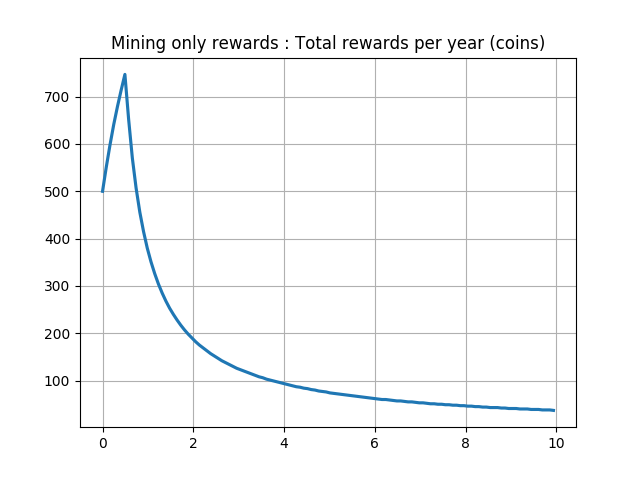
\includegraphics{images/image2.png}}{~}

{}

\begin{center}\rule{0.5\linewidth}{\linethickness}\end{center}

{}

{Rewards Per Year}

{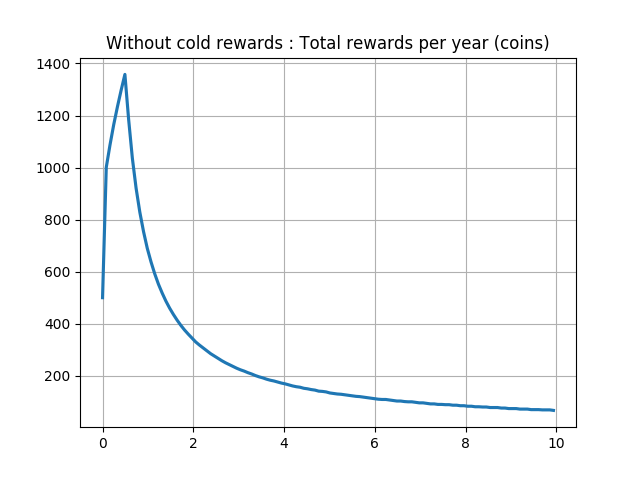
\includegraphics{images/image4.png}}

{Rewards Per Year + Cold Staking*}

{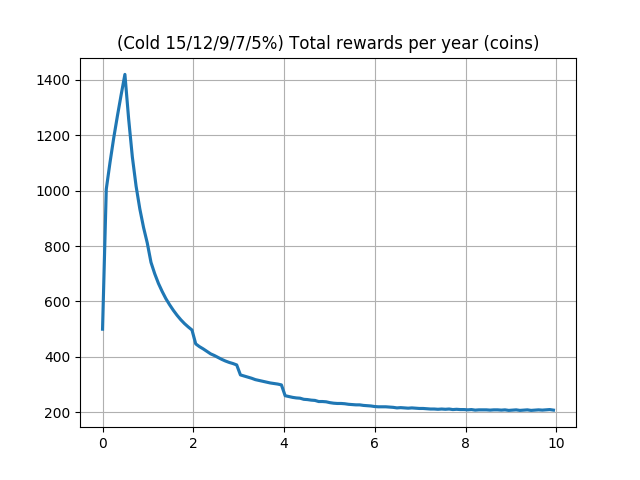
\includegraphics{images/image3.png}}

{}

{*Cold Staking assumes 75\% participation factor.}

{}

{}

{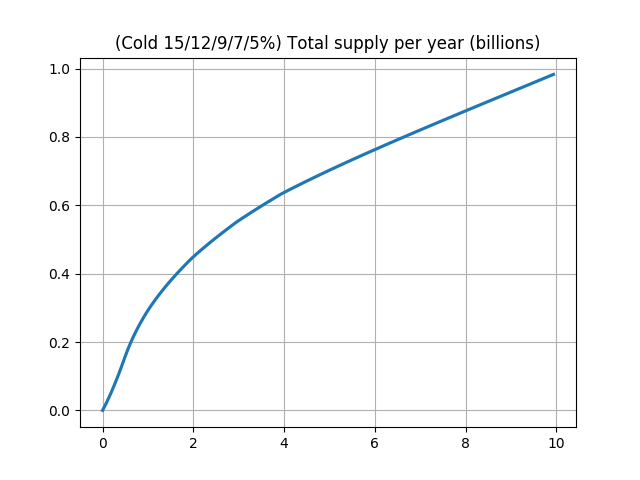
\includegraphics{images/image1.png}}

{}

{}

{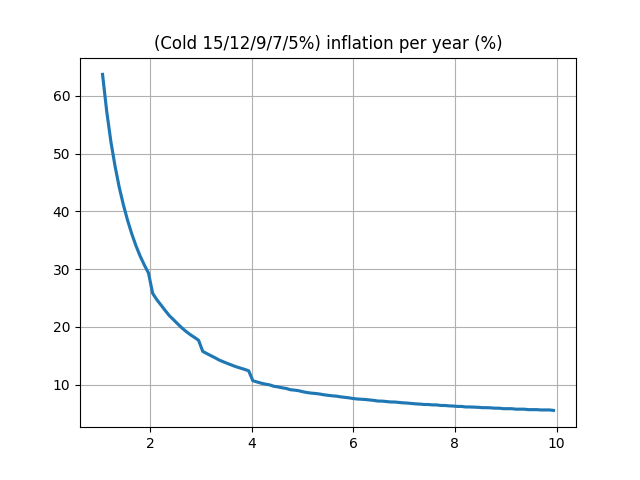
\includegraphics{images/image5.png}}
